\documentclass[11pt,a4paper,reqno,titlepage]{tudelft-light/report}

%Outer Title Page
\begin{document}
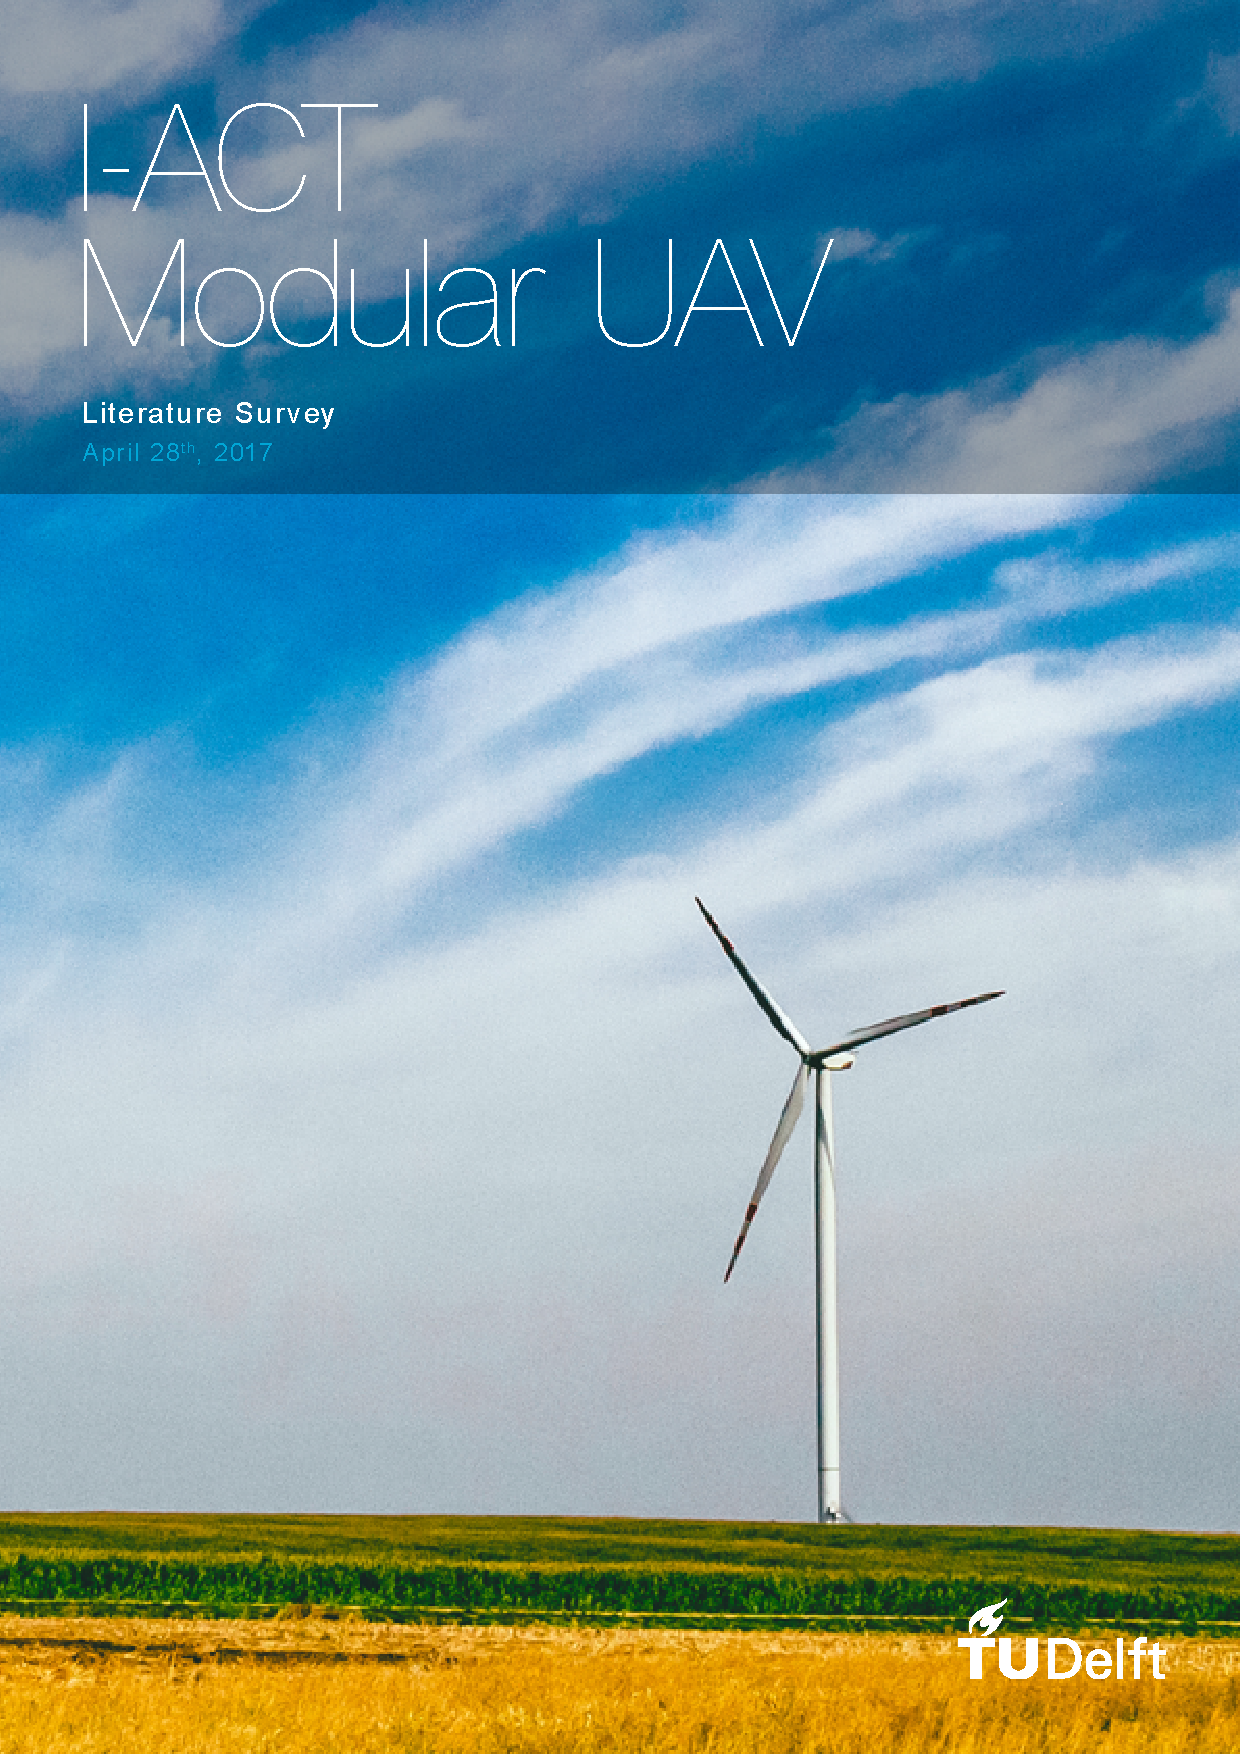
\includepdf[pages={1}]{tudelft-light/title/outercover.pdf}

%Inner Title Page
% TODO Implement a keyword argument style syntax for creating an inner-cover

\newgeometry{margin=6pc} %Change Title-Page Margin Differently
\begin{titlepage}
\begin{center}

\textsc{\LARGE Delft University of Technology}\\[0.25cm]
\textsc{\normalsize [AE4180] Flow Measurement Techniques}\\[1.5cm]

\includegraphics[width=0.25\textwidth]{tudelft-light/title/delft_seal.pdf}\\[1.5cm]
{\huge \bfseries Laboratory Exercise Report} \\
\huge  PIV and HWA Results for a NACA-0012 Airfoil \\[1.0cm]

\begin{minipage}[t]{0.4\textwidth}
\begin{flushleft} \large
\emph{Supervisors:}\\
    Dr. John Doe\\
    

\end{flushleft}
\end{minipage}
\begin{minipage}[t]{0.4\textwidth}
\begin{flushright} \large
\emph{Authors:}\\
    \c{S}. K{\i}lk{\i}\c{s} \textcolor{gray}{4192028}\\
    
\end{flushright}
\end{minipage}\\[2.0cm]

\large \textsc{Abstract}

\begin{minipage}[t]{0.8\textwidth} \large

\blindtext




\end{minipage}

\vfill

\small{\today}

% \small{\textit{Cover Image:} National Aeronautics and Space Administration}\\
% \small{\url{https://www.nasa.gov/sites/default/files/thumbnails/image/airbos_f7_p6.jpg}}

\end{center}
\end{titlepage}
\restoregeometry

%Document Part I: Front matter
\begingroup
\pagenumbering{roman} % Roman page numbers (I, II, III)
    
    %Summary
    %\input{summary} % Summary
    %\addcontentsline{toc}{chapter}{Summary} % Adding the Summary to the ToC

    %Table of Contents
    \renewcommand{\contentsname}{Table of Contents}
    \tableofcontents
    \thispagestyle{empty}
    \setcounter{page}{0}
    \clearpage
    
    %List of Symbols
    \printnomenclature[50pt]

    %List of Figures
    \listoffigures
    \addcontentsline{toc}{chapter}{List of Figures}

    %List of Tables
    \listoftables
    \addcontentsline{toc}{chapter}{List of Tables}
\endgroup
\cleardoublepage

%Document Part II: Main Matter
\begingroup
\pagenumbering{arabic}

    %Chapters:
    \import{examples/}{latex_elements}
    %ADD CHAPTERS HERE

    %References:
    \begingroup % Creates Separate Group from the Report
    \raggedright % Removes Justification
    %\nocite{*} % Disables biblatex from checking if all references are cited
    \cleardoublepage
    \phantomsection
    \addcontentsline{toc}{chapter}{\BibliographyName}
    \printbibliography[title={\BibliographyName}] % Renames Bibliography
    \endgroup

    %Appendices:
    \begin{appendices}
    \chapter{MATLAB Code}
\label{App:MATLAB}

%\\\\\\\\\\\Definining MATLAB Appendix Colors\\\\\\\\\\\\\\\\\\\\\\\\\\\\\\\\\\\\\\\\\\\\\\\\\\\\\\\\\\\\\\\\\\\\\\\\\\
    
\definecolor{mygreen}{RGB}{28,172,0}
\definecolor{mylilas}{RGB}{170,55,241}
\definecolor{mygrey}{RGB}{125,125,125}
\definecolor{myBG}{RGB}{252,252,220}
    
\lstset{language=Matlab,%
    %basicstyle=\color{red},
    breaklines=true,%
    backgroundcolor = \color{myBG},
    morekeywords={matlab2tikz},
    keywordstyle=\color{blue},%
    morekeywords=[2]{1}, keywordstyle=[2]{\color{black}},
    basicstyle=\ttfamily\scriptsize,
    identifierstyle=\color{black}\ttfamily,%
    stringstyle=\color{mylilas}\ttfamily,
    commentstyle=\color{mygreen}\ttfamily,%
    showstringspaces=false,%without this there will be a symbol in the places where there is a space
    numbers=right,%
    numberstyle={\tiny \color{mygrey}},% size of the numbers
    numbersep=9pt, % this defines how far the numbers are from the text
    emph=[1]{NoZ1,NoZ2},emphstyle=[1]\color{cyan}, %Put Global Variables in Here!
} % Loading necessary MATLAB syntax definition for Listings package

\section{Main Script [main.m]}

\lstinputlisting{Appendices/MATLAB/main.m}

\section{Table Look-Up Function [meter2geo.m]}

\lstinputlisting{Appendices/MATLAB/meter2geo.m}
    \end{appendices}
\endgroup
\end{document}